% Options for packages loaded elsewhere
\PassOptionsToPackage{unicode}{hyperref}
\PassOptionsToPackage{hyphens}{url}
\documentclass[
  french,
  10pt,
]{article}
\usepackage{xcolor}
\usepackage[top=2.2cm, bottom=2.4cm, left=2.5cm, right=2.5cm]{geometry}
\usepackage{amsmath,amssymb}
\setcounter{secnumdepth}{5}
\usepackage{iftex}
\ifPDFTeX
  \usepackage[T1]{fontenc}
  \usepackage[utf8]{inputenc}
  \usepackage{textcomp} % provide euro and other symbols
\else % if luatex or xetex
  \usepackage{unicode-math} % this also loads fontspec
  \defaultfontfeatures{Scale=MatchLowercase}
  \defaultfontfeatures[\rmfamily]{Ligatures=TeX,Scale=1}
\fi
\usepackage{lmodern}
\ifPDFTeX\else
  % xetex/luatex font selection
\fi
% Use upquote if available, for straight quotes in verbatim environments
\IfFileExists{upquote.sty}{\usepackage{upquote}}{}
\IfFileExists{microtype.sty}{% use microtype if available
  \usepackage[]{microtype}
  \UseMicrotypeSet[protrusion]{basicmath} % disable protrusion for tt fonts
}{}
\makeatletter
\@ifundefined{KOMAClassName}{% if non-KOMA class
  \IfFileExists{parskip.sty}{%
    \usepackage{parskip}
  }{% else
    \setlength{\parindent}{0pt}
    \setlength{\parskip}{6pt plus 2pt minus 1pt}}
}{% if KOMA class
  \KOMAoptions{parskip=half}}
\makeatother
\usepackage{graphicx}
\makeatletter
\newsavebox\pandoc@box
\newcommand*\pandocbounded[1]{% scales image to fit in text height/width
  \sbox\pandoc@box{#1}%
  \Gscale@div\@tempa{\textheight}{\dimexpr\ht\pandoc@box+\dp\pandoc@box\relax}%
  \Gscale@div\@tempb{\linewidth}{\wd\pandoc@box}%
  \ifdim\@tempb\p@<\@tempa\p@\let\@tempa\@tempb\fi% select the smaller of both
  \ifdim\@tempa\p@<\p@\scalebox{\@tempa}{\usebox\pandoc@box}%
  \else\usebox{\pandoc@box}%
  \fi%
}
% Set default figure placement to htbp
\def\fps@figure{htbp}
\makeatother
\ifLuaTeX
\usepackage[bidi=basic]{babel}
\else
\usepackage[bidi=default]{babel}
\fi
% get rid of language-specific shorthands (see #6817):
\let\LanguageShortHands\languageshorthands
\def\languageshorthands#1{}
\setlength{\emergencystretch}{3em} % prevent overfull lines
\providecommand{\tightlist}{%
  \setlength{\itemsep}{0pt}\setlength{\parskip}{0pt}}
\usepackage{longtable}
\usepackage{booktabs}
\usepackage{array}
\usepackage{multirow}
\usepackage{float}
\usepackage{colortbl}
\usepackage[dvipsnames, table]{xcolor}
\usepackage{caption}
\usepackage{subcaption}
\usepackage{fancyhdr}
\usepackage{graphicx}
\usepackage{wrapfig}
\usepackage{amsmath}
\usepackage{amssymb}
\usepackage{tcolorbox}
\usepackage{mdframed}
\usepackage{enumitem}
\usepackage{makecell}
\usepackage{setspace}
\floatplacement{figure}{H}
\floatplacement{table}{H}
\captionsetup{font=small, labelfont={bf,color=NavyBlue}, skip=4pt}
\captionsetup[table]{position=top}
\definecolor{NavyBlue}{RGB}{0, 51, 102}
\definecolor{SteelBlue}{RGB}{52, 101, 164}
\definecolor{LightBlue}{RGB}{220, 234, 245}
\definecolor{AccentGold}{RGB}{198, 147, 35}
\definecolor{DarkGray}{RGB}{55, 55, 55}
\definecolor{LightGray}{RGB}{245, 246, 248}
\definecolor{SuccessGreen}{RGB}{39, 119, 71}
\definecolor{AlertRed}{RGB}{176, 44, 44}
\definecolor{RowOdd}{RGB}{248, 250, 253}
\definecolor{RowEven}{RGB}{255, 255, 255}
\definecolor{HeaderBg}{RGB}{0, 51, 102}
\pagestyle{fancy}
\fancyhf{}
\fancyhead[L]{\small\textcolor{NavyBlue}{\textbf{Nigeria GHS Panel}} \textcolor{DarkGray}{|} \textit{\small Analyse des superficies agricoles}}
\fancyhead[R]{\small\textcolor{DarkGray}{ENSAE ISE 1 | 2025--2026}}
\fancyfoot[C]{\textcolor{DarkGray}{\thepage}}
\fancyfoot[L]{\textcolor{DarkGray}{\scriptsize\textit{KEBJAM et PARFAIT — ISE 1, 2025-2026}}}
\renewcommand{\headrulewidth}{0.8pt}
\renewcommand{\headrule}{\hbox to\headwidth{\color{NavyBlue}\leaders\hrule height \headrulewidth\hfill}}
\renewcommand{\footrulewidth}{0.3pt}
\renewcommand{\footrule}{\hbox to\headwidth{\color{LightBlue}\leaders\hrule height \footrulewidth\hfill}}
\tcbuselibrary{skins, breakable}
\newtcolorbox{methodbox}[1]{colback=LightBlue!30, colframe=NavyBlue, fonttitle=\bfseries\color{white}, coltitle=white, title=#1, arc=3pt, boxrule=0.8pt, left=6pt, right=6pt, top=4pt, bottom=4pt}
\newtcolorbox{resultbox}[1]{colback=SuccessGreen!8, colframe=SuccessGreen, fonttitle=\bfseries\color{white}, coltitle=white, title=#1, arc=3pt, boxrule=0.8pt, left=6pt, right=6pt, top=4pt, bottom=4pt}
\newtcolorbox{alertbox}[1]{colback=AlertRed!8, colframe=AlertRed, fonttitle=\bfseries\color{white}, coltitle=white, title=#1, arc=3pt, boxrule=0.8pt, left=6pt, right=6pt, top=4pt, bottom=4pt}
\setlength{\parskip}{4pt}
\setlength{\parindent}{0pt}
\usepackage{bookmark}
\IfFileExists{xurl.sty}{\usepackage{xurl}}{} % add URL line breaks if available
\urlstyle{same}
\hypersetup{
  pdflang={fr},
  hidelinks,
  pdfcreator={LaTeX via pandoc}}

\title{\vspace{-1cm}
\textcolor{NavyBlue}{\rule{\linewidth}{2pt}}
\vspace{0.3cm}

\textbf{TP 4 -- Analyse des parcelles agricoles : superficie, tenure foncière et utilisation des terres}\textbackslash{}
\large\textit{Nigeria General Household Survey (2018)} \vspace{0.2cm}

\textcolor{NavyBlue}{\rule{\linewidth}{0.5pt}}}
\author{\textbf{Groupe 7 : KEBJAM Jackson et NGOYI Parfait Jemmy Prodige — ISE 1, 2025-2026}}
\date{17 avril 2026}

\begin{document}
\maketitle

{
\setcounter{tocdepth}{3}
\tableofcontents
}
\section{Introduction}\label{introduction}

Le secteur agricole occupe une place centrale dans l'économie nigériane.
Il emploie près de 35 \% de la population active et contribue de manière
significative au produit intérieur brut du pays. Comprendre les
structures foncières, les modes d'exploitation et les disparités
régionales est essentiel pour éclairer les politiques publiques en
matière de sécurité alimentaire, de développement rural et de lutte
contre la pauvreté.

Cette étude s'appuie sur la vague 4 (2018-2019) du Nigeria General
Household Survey (GHS) Panel, une enquête menée par la Banque mondiale
en collaboration avec le Bureau national des statistiques du Nigeria.
L'unité d'analyse retenue est la parcelle agricole, définie comme une
portion de terre délimitée et cultivée par un ménage.

Notre objectif est triple. Premièrement, nous évaluons la qualité des
données déclaratives en identifiant les valeurs manquantes et
aberrantes. Deuxièmement, nous réalisons une analyse statistique
descriptive des superficies agricoles, en intégrant les poids de sondage
pour garantir la représentativité des résultats. Troisièmement, nous
explorons les déterminants de la structure foncière, notamment le régime
de tenure, la fragmentation des exploitations et les disparités
géographiques entre les États du Nigeria.

\section{VALEURS MANQUANTES et ABERRANTES
(Q19)}\label{valeurs-manquantes-et-aberrantes-q19}

\section{Présentation des données}\label{intro}

L'analyse mobilise quatre fichiers complémentaires issus de la vague 4.
Le fichier section a harvest fournit les variables de stratification et
les poids de sondage nécessaires à l'inférence statistique. Le fichier
section a1 harvest contient les superficies déclarées par les
exploitants ainsi que les mesures GPS de référence. Les fichiers section
11 a1 planting et section 11 b1 planting renseignent respectivement les
superficies exprimées en unités locales (heaps, ridges, stands) et les
modes d'acquisition foncière. La jointure entre ces sources s'effectue
grâce aux identifiants ménage et parcelle.

\subsection{Description des sources de
données}\label{description-des-sources-de-donnuxe9es}

\{ \footnotesize \rowcolors{2}{RowOdd}{white}

\begin{table}

\caption{\label{tab:desc-sources-table}Sources de données --- Nigeria GHS Wave 4}
\centering
\begin{tabular}[t]{llll}
\toprule
\cellcolor{NavyBlue}\textcolor{white}{\textbf{Fichier}} & \cellcolor{NavyBlue}\textcolor{white}{\textbf{Contenu principal}} & \cellcolor{NavyBlue}\textcolor{white}{\textbf{Variables clés}} & \cellcolor{NavyBlue}\textcolor{white}{\textbf{Jointure}}\\
\midrule
secta\_harvestw4 & Stratification, poids de sondage & hhid, zone, state, sector, wt\_wave4 & Base principale\\
secta1\_harvestw4 & Superficie déclarée, mesure GPS & plotid, sa1q11, prefilled\_gps\_area & by = hhid\\
sect11a1\_plantingw4 & Superficie en unités locales & s11aq4aa, s11aq4b & by = hhid + plotid\\
sect11b1\_plantingw4 & Mode d'acquisition foncière & s11b1q4 & by = hhid + plotid\\
\bottomrule
\end{tabular}
\end{table}

\}

\subsection{Construction de la variable superficie en
hectares}\label{methodo-superficie}

La principale difficulté méthodologique réside dans l'hétérogénéité des
unités de mesure déclarées par les ménages. Trois cas de figure se
présentent. Pour les unités standardisées, nous appliquons des facteurs
de conversion fixes : un hectare correspond à lui-même , un acre est
converti en hectares par multiplication par 0,404686 , et un mètre carré
est divisé par 10 000 .

Les unités locales --- heaps (tassements de terre pour tubercules),
ridges (billons de culture) et stands (pieds de culture) --- posent un
défi plus complexe car leur équivalence en hectares varie selon la zone
géographique. Nous appliquons les facteurs de conversion régionaux
fournis par le protocole LSMS-ISA de la Banque mondiale. Par exemple,
dans la zone North West, un ridge correspond à 0,00494 hectare, tandis
que dans le South West, le même ridge n'équivaut qu'à 0,00001 hectare.
Ces variations reflètent les différences dans les pratiques culturales
et la densité des plantations.

La superficie finale est construite par l'opérateur qui retient la
première valeur non manquante dans l'ordre hiérarchique suivant : unités
standard, heaps, ridges, stands. Parallèlement, la mesure GPS, exprimée
en mètres carrés, est convertie en hectares par division par 10 000.

\subsubsection{Unités standard}\label{unituxe9s-standard}

\begin{equation}
\text{superficie\_ha} = \begin{cases}
\text{superficie} \times 1 & \text{si unité} = \text{Hectares (code 6)} \\[4pt]
\text{superficie} \times 0.404686 & \text{si unité} = \text{Acres (code 5)} \\[4pt]
\dfrac{\text{superficie}}{10\,000} & \text{si unité} = \text{Mètres carrés (code 7)}
\end{cases}
\end{equation}

\subsubsection{Unités locales --- facteurs de conversion
régionaux}\label{unituxe9s-locales-facteurs-de-conversion-ruxe9gionaux}

\{ \small \rowcolors{2}{RowOdd}{white}

\begin{table}

\caption{\label{tab:table-conversion}Facteurs de conversion régionaux (ha/unité) --- source : LSMS-ISA, World Bank}
\centering
\begin{tabular}[t]{lrrr}
\toprule
\cellcolor{NavyBlue}\textcolor{white}{\textbf{Zone géographique}} & \cellcolor{NavyBlue}\textcolor{white}{\textbf{Heaps (ha/heap)}} & \cellcolor{NavyBlue}\textcolor{white}{\textbf{Ridges (ha/ridge)}} & \cellcolor{NavyBlue}\textcolor{white}{\textbf{Stands (ha/stand)}}\\
\midrule
North Central (1) & 0.00012 & 0.0027 & 0.00006\\
North East (2) & 0.00016 & 0.0040 & 0.00016\\
North West (3) & 0.00011 & 0.00494 & 0.00004\\
South East (4) & 0.00019 & 0.0023 & 0.00004\\
South South (5) & 0.00021 & 0.0023 & 0.00013\\
South West (6) & 0.00012 & 0.00001 & 0.00041\\
\bottomrule
\end{tabular}
\end{table}
\vspace{2pt}

\{\footnotesize\textit{Note : Heap : tubercules (igname, manioc). Ridge : billons de culture. Stand : pied de culture.}\}
\}

\subsubsection{Règle de fusion et contrôle
qualité}\label{ruxe8gle-de-fusion-et-contruxf4le-qualituxe9}

Pour garantir la fiabilité de l'analyse, nous appliquons une règle
d'exclusion systématique : toute parcelle dont la superficie est
inférieure ou égale à zéro hectare (erreur de saisie ou unité manquante)
ou supérieure à 500 hectares (valeur extrême vraisemblablement due à une
erreur de conversion) est temporairement exclue de l'analyse principale.
Ces observations sont néanmoins conservées dans la base brute,
permettant d'en conserver la trace pour d'éventuelles analyses de
sensibilité.

L'examen des valeurs manquantes révèle des disparités importantes selon
les variables. La variable superficie déclarée présente le taux de
manquants le plus élevé, avec 1 104 observations absentes sur 12 114
parcelles, soit 9,1 \% de données manquantes. Ce taux élevé s'explique
probablement par des erreurs de saisie ou des non-réponses partielles
lors de l'enquête. En revanche, les variables issues du module planting
(superficie parcelle, superficie convertie) affichent un taux de
renseignement satisfaisant de 90,5 \%. Le poids de sondage, élément
critique pour l'inférence, est quasi exhaustif avec 99,6 \% de valeurs
renseignées.

S'agissant des valeurs aberrantes, nous observons qu'aucune parcelle ne
présente de superficie nulle ou négative dans la base nettoyée, ce qui
atteste de l'efficacité des filtres appliqués en amont. Cinq parcelles
seulement dépassent le seuil de 500 hectares, représentant 0,04 \% de
l'échantillon, et sont exclues de l'analyse principale. Au total, 10 956
parcelles (90,4 \% de l'échantillon initial) sont retenues pour
l'analyse univariée. Ce taux de rétention est satisfaisant et permet de
garantir la robustesse des estimations.

\section{Qualité des données : valeurs manquantes et
aberrantes}\label{tache19}

\{ \small \rowcolors{2}{RowOdd}{white}

\begin{table}

\caption{\label{tab:missing-table}Diagnostic des valeurs manquantes --- Nigeria GHS W4 (N = 12 114 parcelles)}
\centering
\begin{tabular}[t]{lrrrr}
\toprule
\cellcolor{NavyBlue}\textcolor{white}{\textbf{Variable}} & \cellcolor{NavyBlue}\textcolor{white}{\textbf{N manquants}} & \cellcolor{NavyBlue}\textcolor{white}{\textbf{\% manquants}} & \cellcolor{NavyBlue}\textcolor{white}{\textbf{N renseignés}} & \cellcolor{NavyBlue}\textcolor{white}{\textbf{\% renseignés}}\\
\midrule
Superficie déclarée (sa1q11) & 11048 & 91.2 & 1066 & 8.8\\
Superficie parcelle (s11aq4aa) & 1153 & 9.5 & 10961 & 90.5\\
Superficie convertie (area\_ha) & 1153 & 9.5 & 10961 & 90.5\\
Superficie nettoyée (area\_ha\_propre) & 1158 & 9.6 & 10956 & 90.4\\
Superficie GPS (ha) & 5287 & 43.6 & 6827 & 56.4\\
Poids de sondage (wt\_wave4) & 49 & 0.4 & 12065 & 99.6\\
\bottomrule
\end{tabular}
\end{table}

\}

\{ \small \rowcolors{2}{RowOdd}{white}

\begin{table}

\caption{\label{tab:outliers-table}Distribution des valeurs aberrantes --- variable superficie en ha}
\centering
\begin{tabular}[t]{lrrc}
\toprule
\cellcolor{NavyBlue}\textcolor{white}{\textbf{Catégorie}} & \cellcolor{NavyBlue}\textcolor{white}{\textbf{N}} & \cellcolor{NavyBlue}\textcolor{white}{\textbf{\%}} & \cellcolor{NavyBlue}\textcolor{white}{\textbf{Statut}}\\
\midrule
Valeur nulle ($= 0$ ha) & 0 & NaN & Exclu\\
Valeur négative ($< 0$ ha) & 0 & NaN & Exclu\\
Valeur aberrante ($> 500$ ha) & 5 & 100 & Exclu\\
Valeur manquante (NA) & 1153 & 100 & Exclu\\
\textbf{Valeur valide} ($0 <$ ha $\leq 500$) & 10956 & 100 & \textcolor{SuccessGreen}{Retenu}\\
\bottomrule
\end{tabular}
\end{table}

\}

\section{ANALYSE UNIVARIÉE (Q20)}\label{analyse-univariuxe9e-q20}

\section{Analyse univariée pondérée des superficies}\label{tache20}

Toutes les analyses sont rigoureusement pondérées par le poids de
sondage afin de restituer la représentativité nationale.

\subsection{Statistiques descriptives
pondérées}\label{statistiques-descriptives-ponduxe9ruxe9es}

\{ \small \rowcolors{2}{RowOdd}{white}

\begin{table}

\caption{\label{tab:stats-table}Statistiques descriptives pondérées --- Superficies agricoles, Nigeria GHS W4}
\centering
\begin{tabular}[t]{lrrrrrrrrr}
\toprule
\cellcolor{NavyBlue}\textcolor{white}{\textbf{Indicateur}} & \cellcolor{NavyBlue}\textcolor{white}{\textbf{$N$}} & \cellcolor{NavyBlue}\textcolor{white}{\textbf{Moy.}} & \cellcolor{NavyBlue}\textcolor{white}{\textbf{Méd.}} & \cellcolor{NavyBlue}\textcolor{white}{\textbf{Éc.-type}} & \cellcolor{NavyBlue}\textcolor{white}{\textbf{$Q_1$}} & \cellcolor{NavyBlue}\textcolor{white}{\textbf{$Q_3$}} & \cellcolor{NavyBlue}\textcolor{white}{\textbf{Min}} & \cellcolor{NavyBlue}\textcolor{white}{\textbf{Max}} & \cellcolor{NavyBlue}\textcolor{white}{\textbf{CV (\%)}}\\
\midrule
Superficie / parcelle (ha) & 10955 & 0.642 & 0.320 & 3.053 & 0.057 & 0.809 & 0 & 480.000 & 475.5\\
Superficie totale / ménage (ha) & 3869 & 1.756 & 0.879 & 7.091 & 0.287 & 2.023 & 0 & 480.649 & 403.8\\
\bottomrule
\end{tabular}
\end{table}

\}

Les résultats révèlent une structure foncière profondément inégalitaire.
Au niveau parcellaire, la superficie médiane s'établit à 0,32 hectare,
tandis que la moyenne atteint 0,64 hectare. Cette différence
significative entre médiane et moyenne indique une asymétrie positive
marquée : une majorité de petites parcelles coexiste avec une minorité
de grandes exploitations qui tirent la moyenne vers le haut.

\subsection{Distribution des superficies (échelle
logarithmique)}\label{distribution-des-superficies-uxe9chelle-logarithmique}

La transformation logarithmique \(\ln(1 + x)\) qui permet d'inclure les
valeurs nulles sans produire de valeurs infinies, visualise clairement
cette dualité structurale. L'histogramme des superficies par parcelle
montre une masse importante d'observations concentrée en dessous de 0,5
hectare, correspondant aux exploitations de subsistance. Un second mode,
moins dense mais présent, s'étend au-delà de 5 hectares. La distribution
par ménage amplifie ce phénomène, avec une queue de distribution encore
plus étirée vers les grandes surfaces.

\begin{figure}[H]
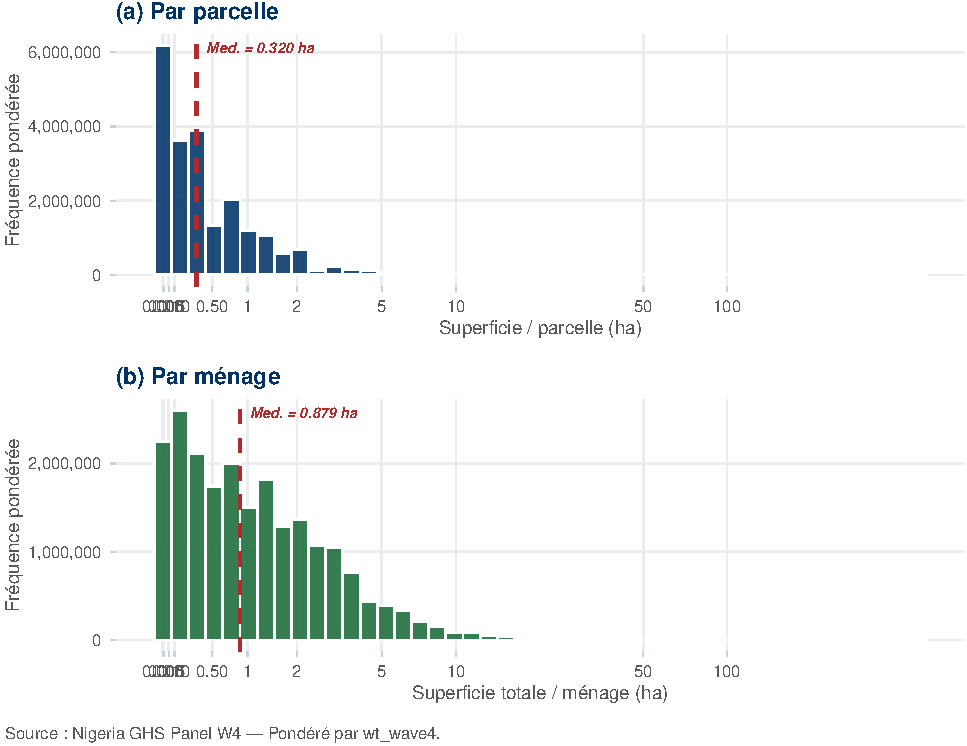
\includegraphics[width=1\linewidth]{rapport_final_files/figure-latex/histogrammes-1} \caption{Distribution pondérée des superficies agricoles. Transformation $\ln(1 + x)$. Ligne rouge = médiane pondérée.}\label{fig:histogrammes}
\end{figure}

\subsection{Boxplots}\label{boxplots}

Cette asymétrie s'accentue au niveau du ménage. La superficie totale
médiane par ménage est de 0,88 hectare, alors que la moyenne s'élève à
1,76 hectare, soit plus du double. Le coefficient de variation, qui
atteint 404 \% au niveau ménage, confirme l'extrême hétérogénéité des
structures foncières nigérianes. En d'autres termes, la dispersion
autour de la moyenne est considérable, traduisant une concentration des
terres entre les mains d'une minorité de grands exploitants.

\begin{figure}[H]
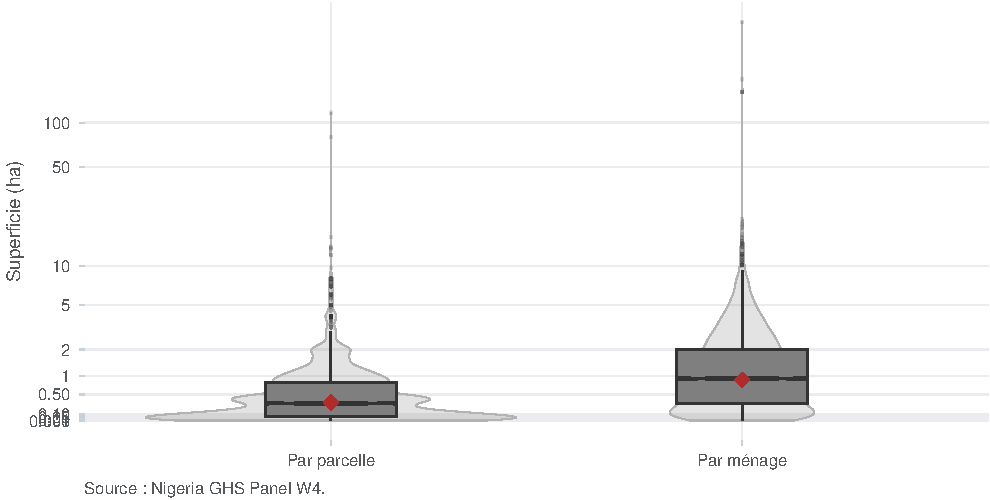
\includegraphics[width=1\linewidth]{rapport_final_files/figure-latex/boxplot-1} \caption{Boxplots des superficies agricoles (rééchantillonnage pondéré, $n=4000$).}\label{fig:boxplot}
\end{figure}

\subsection{Déciles pondérés}\label{duxe9ciles-ponduxe9ruxe9s}

L'analyse par déciles apporte un éclairage complémentaire sur cette
concentration. Les 10 \% des ménages les plus petits (Décile 1)
cultivent en moyenne 0,028 hectare et ne contribuent qu'à 0,2 \% de la
superficie totale pondérée. À l'opposé, les 10 \% des ménages les plus
grands (Décile 10) exploitent en moyenne 8,17 hectares et concentrent 10
\% de la superficie totale. La borne supérieure du Décile 10 atteint
480,65 hectares, attestant de l'existence d'une agriculture commerciale
de grande échelle coexistant avec une agriculture familiale de
subsistance.

\{ \small \rowcolors{2}{RowOdd}{white}

\begin{table}

\caption{\label{tab:deciles}Statistiques pondérées par décile --- superficie totale par ménage (W4)}
\centering
\begin{tabular}[t]{lrrrrr}
\toprule
\cellcolor{NavyBlue}\textcolor{white}{\textbf{Décile}} & \cellcolor{NavyBlue}\textcolor{white}{\textbf{N}} & \cellcolor{NavyBlue}\textcolor{white}{\textbf{Borne inf. (ha)}} & \cellcolor{NavyBlue}\textcolor{white}{\textbf{Borne sup. (ha)}} & \cellcolor{NavyBlue}\textcolor{white}{\textbf{Moy. pond. (ha)}} & \cellcolor{NavyBlue}\textcolor{white}{\textbf{Part (\%)}}\\
\midrule
D1 & 349 & 0.000 & 0.065 & 0.028 & 10.0\\
D2 & 394 & 0.065 & 0.200 & 0.129 & 10.0\\
D3 & 350 & 0.200 & 0.405 & 0.287 & 9.3\\
D4 & 403 & 0.405 & 0.617 & 0.486 & 10.7\\
D5 & 357 & 0.617 & 0.879 & 0.770 & 10.0\\
D6 & 401 & 0.879 & 1.218 & 1.074 & 10.0\\
D7 & 392 & 1.218 & 1.731 & 1.469 & 9.9\\
D8 & 439 & 1.731 & 2.451 & 2.082 & 10.1\\
D9 & 373 & 2.451 & 3.700 & 3.028 & 10.0\\
D10 & 411 & 3.700 & 480.649 & 8.172 & 10.0\\
\bottomrule
\end{tabular}
\end{table}

\}

\section{Comparaison superficie déclarée et GPS}\label{gps}

\begin{methodbox}{Enjeu méthodologique}
La confrontation entre la superficie déclarée oralement par les exploitants et la mesure GPS objective constitue un enjeu méthodologique central. Les déclarations orales sont susceptibles de biais cognitifs : arrondis systématiques, sous-déclaration des grandes parcelles par crainte fiscale, ou surestimation par attachement psychologique à la terre. La corrélation de Spearman est préférée au coefficient de Pearson car elle est robuste aux valeurs extrêmes et ne suppose pas la normalité des distributions.
\end{methodbox}

\subsection{Statistiques du biais de
déclaration}\label{statistiques-du-biais-de-duxe9claration}

L'analyse porte sur 6 822 paires d'observations valides. La corrélation
de Spearman atteint 0,7021, ce qui témoigne d'une forte concordance en
rang entre les deux mesures : les exploitants perçoivent correctement
l'ordre de grandeur relatif de leurs parcelles (la parcelle A est plus
grande que la parcelle B).

Cependant, le biais médian (GPS - déclaré) est de -0,0264 hectare, ce
qui signifie que la superficie déclarée excède systématiquement la
mesure GPS. En d'autres termes, les exploitants ont tendance à
surestimer leurs propres parcelles. Ce résultat est cohérent avec la
littérature internationale (Carletto et al., 2015), qui attribue ce
biais à une combinaison de facteurs : arrondis psychologiques,
méconnaissance des unités standardisées, et réticence à déclarer des
petites surfaces perçues comme socialement dévalorisantes.

La proportion de parcelles sous-estimées (déclaré \(>\) GPS) atteint
38,7 \%, tandis que 61,3 \% des parcelles sont sur-estimées (déclaré
\(<\) GPS). Ce déséquilibre suggère que le biais n'est pas symétrique :
la surestimation est plus fréquente que la sous-estimation.

\{ \small \rowcolors{2}{RowOdd}{white}

\begin{table}

\caption{\label{tab:biais-table}Statistiques du biais de déclaration --- superficie GPS vs. déclarée (W4)}
\centering
\begin{tabular}[t]{lrl}
\toprule
\cellcolor{NavyBlue}\textcolor{white}{\textbf{Indicateur}} & \cellcolor{NavyBlue}\textcolor{white}{\textbf{Valeur}} & \cellcolor{NavyBlue}\textcolor{white}{\textbf{Interprétation}}\\
\midrule
Paires (déclaré, GPS) valides & 6 822 & Observations appariées\\
Corrélation de Spearman ($\rho$) & 0.7021 & Forte concordance\\
Biais moyen (GPS $-$ déclaré) & -0.1428 ha & Sur-déclaration en moyenne\\
Biais médian (GPS $-$ déclaré) & -0.0264 ha & Sur-déclaration médiane\\
Part sous-estimée (déclaré $>$ GPS) & 38.7 \% & Exploitants déclarant plus que le GPS\\
Part sur-estimée (déclaré $<$ GPS) & 61.3 \% & Exploitants déclarant moins que le GPS\\
\bottomrule
\end{tabular}
\end{table}

\}

\subsection{Scatter plot avec hexagones de
densité}\label{scatter-plot-avec-hexagones-de-densituxe9}

Le scatter plot en hexagones de densité confirme visuellement ces
résultats. La ligne d'égalité parfaite (biais nul) est systématiquement
dépassée par le nuage de points dans la zone des petites surfaces
(inférieures à 1 hectare), où la densité d'observations est maximale. La
courbe LOESS, qui lisse la relation moyenne entre les deux mesures,
s'écarte nettement de la ligne d'égalité pour les surfaces inférieures à
2 hectares, confirmant la surestimation systématique. Pour les grandes
surfaces (supérieures à 5 hectares), l'incertitude augmente, comme en
témoigne l'élargissement de l'intervalle de confiance.

Implication politique : toute politique agricole basée sur les seules
déclarations orales surestimera systématiquement les superficies
cultivées, conduisant à une allocation inefficace des subventions et des
conseils agricoles. La généralisation de la mesure GPS dans les enquêtes
futures est donc impérative.

\begin{figure}[H]
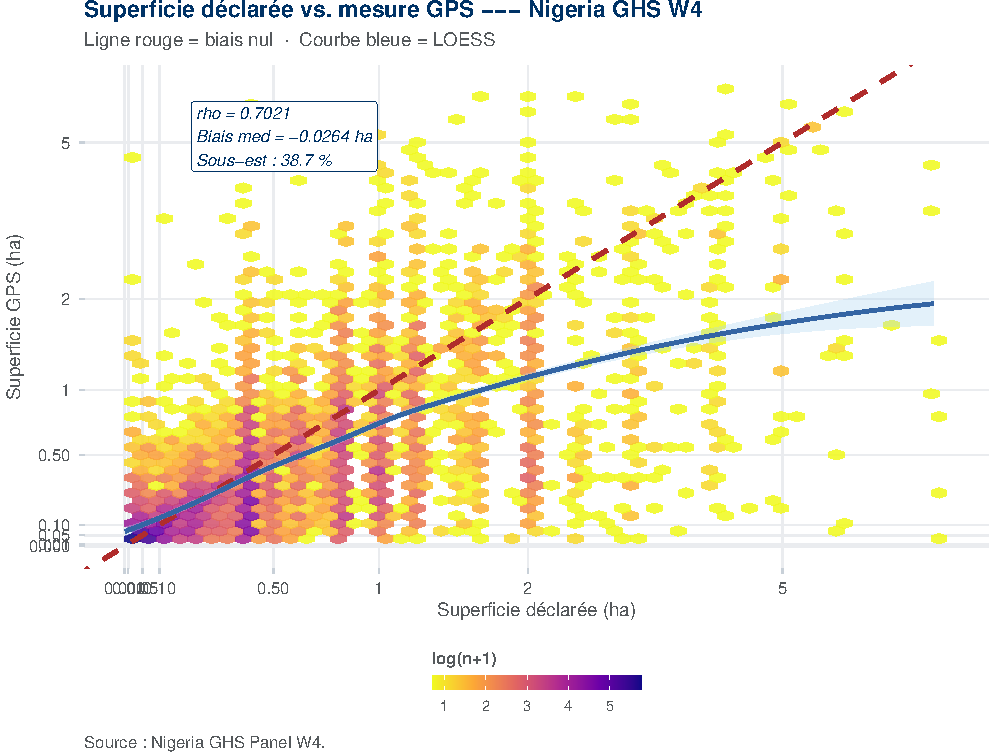
\includegraphics[width=1\linewidth]{rapport_final_files/figure-latex/scatter-gps-1} \caption{Superficie déclarée vs. superficie GPS. Ligne rouge = biais nul ; courbe bleue = LOESS.}\label{fig:scatter-gps}
\end{figure}

\textbf{Interprétation.} La corrélation de Spearman (\(\rho =\) 0.7021)
indique une bonne concordance en rang. Cependant, 38.7\% des parcelles
présentent une \textbf{sous-déclaration}, avec un biais médian de
-0.0264 ha (Carletto \emph{et al.}, 2015).

\section{MODE D'ACQUISITION
(TENURE)(Q21)}\label{mode-dacquisition-tenureq21}

\section{Régime de tenure foncière}\label{tache21}

L'analyse des modes d'acquisition foncière révèle la prédominance
écrasante du régime d'héritage, qui concerne 63 \% des parcelles en
termes bruts et 58,2 \% en termes pondérés. Ce résultat reflète la
persistance des systèmes coutumiers de transmission foncière au Nigeria,
où la terre est perçue comme un patrimoine familial inaliénable plutôt
que comme une marchandise.

Le second régime le plus fréquent est la propriété pleine (achat), qui
représente 15,6 \% des parcelles pondérées, suivie de la location (12,9
\%) et du prêt (9,7 \%). Les autres modes --- communautaire (2,6 \%),
métayage (0,6 \%) et échange temporaire (0,4 \%) --- jouent un rôle
marginal. Cette structure suggère que le marché foncier formel reste peu
développé, et que l'accès à la terre repose principalement sur les
réseaux familiaux et communautaires.

\{ \small \rowcolors{2}{RowOdd}{white}

\begin{table}

\caption{\label{tab:tenure-table}Régimes de tenure foncière --- fréquences brutes et pondérées, Nigeria GHS W4}
\centering
\begin{tabular}[t]{lrrrrr}
\toprule
\cellcolor{NavyBlue}\textcolor{white}{\textbf{Tenure}} & \cellcolor{NavyBlue}\textcolor{white}{\textbf{N brut}} & \cellcolor{NavyBlue}\textcolor{white}{\textbf{Eff. pond.}} & \cellcolor{NavyBlue}\textcolor{white}{\textbf{\% brut}} & \cellcolor{NavyBlue}\textcolor{white}{\textbf{\% pond.}} & \cellcolor{NavyBlue}\textcolor{white}{\textbf{\% cum.}}\\
\midrule
héritage & 6906 & 12462724 & 63.0 & 58.2 & 99.0\\
propriété pleine & 1268 & 3343792 & 11.6 & 15.6 & 15.6\\
location & 1218 & 2759370 & 11.1 & 12.9 & 28.5\\
prêt & 1002 & 2085777 & 9.1 & 9.7 & 38.2\\
communautaire & 455 & 561872 & 4.2 & 2.6 & 40.8\\
métayage & 68 & 123569 & 0.6 & 0.6 & 99.6\\
échange temporaire & 43 & 68809 & 0.4 & 0.3 & 99.9\\
\bottomrule
\end{tabular}
\end{table}

\}

\begin{figure}[H]
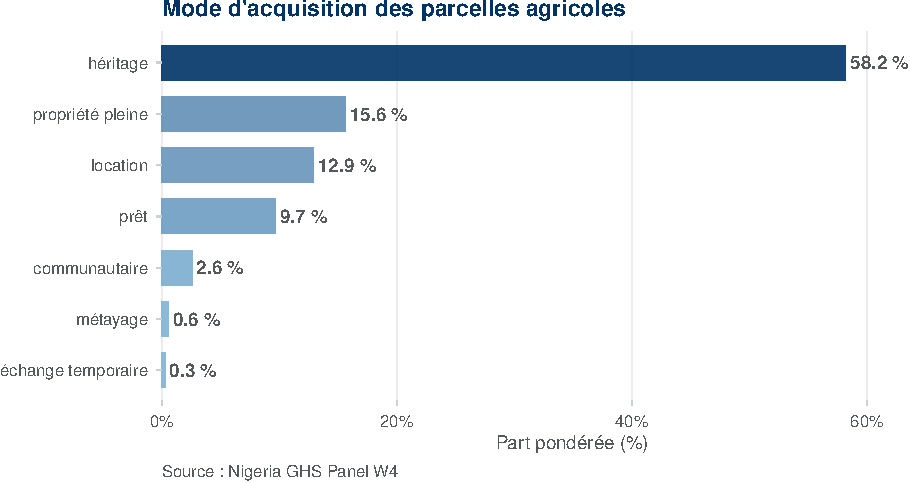
\includegraphics[width=1\linewidth]{rapport_final_files/figure-latex/tenure-barplot-1} \caption{Distribution pondérée des régimes de tenure foncière (Nigeria GHS W4).}\label{fig:tenure-barplot}
\end{figure}

\subsection{\texorpdfstring{Test d'indépendance : tenure \(\times\) zone
de
résidence}{Test d'indépendance : tenure \textbackslash times zone de résidence}}\label{test-dinduxe9pendance-tenure-times-zone-de-ruxe9sidence}

Le test du \(\chi^2\) pondéré, bien qu'approximé (effectifs pondérés
arrondis), révèle une association significative (p\$\textless\$0,001)
entre le régime de tenure et la zone de résidence (rural vs.~urbain). La
valeur du V de Cramér (0,2236) indique une association d'intensité
faible à modérée. En pratique, cela signifie que les modes d'acquisition
diffèrent entre les campagnes et les villes : l'héritage domine
davantage en milieu rural, tandis que la location et l'achat sont plus
fréquents dans les zones urbaines périphériques.

Limite méthodologique : pour une inférence rigoureuse tenant compte du
plan de sondage stratifié, il conviendrait d'utiliser le test de
Rao-Scott. L'approche actuelle, basée sur des effectifs pondérés
arrondis, constitue une approximation raisonnable mais non définitive.

\{ \small \rowcolors{2}{RowOdd}{white}

\begin{table}

\caption{\label{tab:chi2-result}Test du $\chi^2$ pondéré approx. --- tenure $\times$ zone (Rural/Urbain)}
\centering
\begin{tabular}[t]{lr}
\toprule
\cellcolor{NavyBlue}\textcolor{white}{\textbf{Paramètre}} & \cellcolor{NavyBlue}\textcolor{white}{\textbf{Valeur}}\\
\midrule
Statistique $X^2$ & 1070144.859\\
Degrés de liberté ($df$) & 6\\
$p$-value & <0.001\\
V de Cramér & 0.2236\\
Interprétation de l'effet & faible\\
\bottomrule
\end{tabular}
\end{table}

\}

\section{SUPERFICIE TOTALE et NOMBRE DE PARCELLES
(Q23)}\label{superficie-totale-et-nombre-de-parcelles-q23}

La fragmentation des exploitations --- c'est-à-dire la division de la
superficie totale d'un ménage en plusieurs parcelles géographiquement
distinctes --- est une caractéristique majeure de l'agriculture
ouest-africaine. La corrélation de Spearman entre le nombre de parcelles
et la superficie totale atteint 0,433, ce qui correspond à une
association modérée positive.

Cette corrélation positive confirme l'intuition intuitive : les ménages
qui détiennent plus de parcelles cultivent globalement plus de surface.
Cependant, l'intensité modérée de la corrélation (loin de 1) indique que
le nombre de parcelles n'est pas un prédicteur parfait de la superficie
totale. Autrement dit, il existe des ménages avec peu de parcelles mais
de grande taille, et inversement des ménages avec de nombreuses
parcelles de très petite taille.

\{ \small \rowcolors{2}{RowOdd}{white}

\begin{table}

\caption{\label{tab:spearman-table}Corrélation de Spearman --- superficie totale $\times$ nombre de parcelles}
\centering
\begin{tabular}[t]{lr}
\toprule
\cellcolor{NavyBlue}\textcolor{white}{\textbf{Indicateur}} & \cellcolor{NavyBlue}\textcolor{white}{\textbf{Valeur}}\\
\midrule
$\rho$ de Spearman & 0.433\\
Interprétation & Association modérée positive\\
$N$ ménages analysés & 3869\\
\bottomrule
\end{tabular}
\end{table}

\}

La courbe LOESS pondérée, qui lisse la relation moyenne entre les deux
variables, révèle une progression décroissante : chaque parcelle
additionnelle contribue moins à la superficie totale au-delà de 8 à 10
parcelles. Ce phénomène s'explique par la logique de diversification
agricole : les ménages ajoutent d'abord des parcelles de grande taille
pour augmenter leur production vivrière, puis des parcelles secondaires
de petite taille destinées à des cultures de rente (cacao, palmier à
huile) ou à la diversification du risque climatique.

La fragmentation peut avoir des effets ambivalents sur la productivité.
D'un côté, elle permet de cultiver des sols aux caractéristiques
complémentaires (terres basses humides pour le riz, terres hautes pour
le maïs) et de lisser le risque de mauvaises récoltes. De l'autre côté,
elle accroît les coûts de transport, de surveillance et de gestion.

\begin{figure}[H]
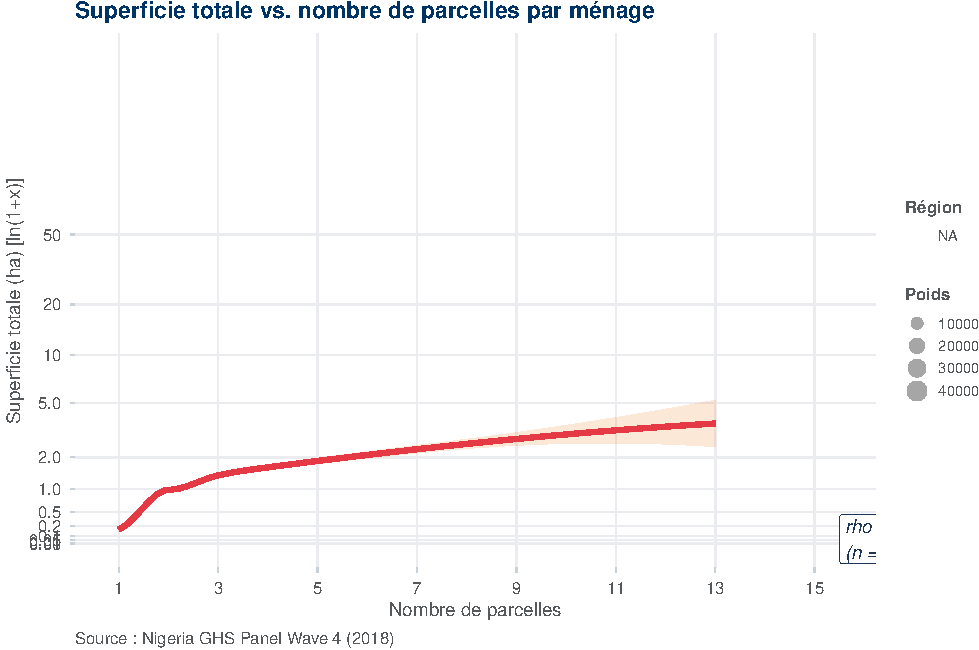
\includegraphics[width=1\linewidth]{rapport_final_files/figure-latex/loess-plot-1} \caption{Superficie totale par ménage en fonction du nombre de parcelles. Courbe LOESS pondérée.}\label{fig:loess-plot}
\end{figure}

\section{CARTE DU NIGERIA (cartographier les disparités géographiques)
(Q24)}\label{carte-du-nigeria-cartographier-les-disparituxe9s-guxe9ographiques-q24}

La heatmap des superficies médianes par État révèle un contraste
Nord-Ouest / Sud-Est systématique. L'État de Nasarawa se distingue
nettement avec la superficie médiane la plus élevée du pays (1,62 ha),
suivi de Katsina (0,81 ha). Un groupe d'États affiche des superficies
comprises entre 0,49 et 0,81 ha : Rivers, Borno, Adamawa, le Territoire
de la capitale fédérale (Abuja), Osun, Kogi, Yobe, Imo et Ogun. De très
nombreux États - Zamfara, Taraba, Sokoto, Oyo, Ondo, Niger, Lagos,
Jigawa, Kano, Kaduna, Ekiti, Bauchi, Delta, Kebbi et Benue --- se
situent précisément à 0,40 ha, ce qui semble constituer une norme
culturale nationale. À l'opposé, les États du Sud-Est et quelques États
du Nord-Est présentent les superficies les plus réduites : Kwara (0,30
ha), Abia (0,26 ha), Ebonyi (0,24 ha), Cross River (0,21 ha), Akwa Ibom
(0,12 ha), Anambra (0,10 ha), Enugu (0,09 ha), Plateau (0,06 ha) et
Gombe (0,04 ha), qui affiche la plus faible superficie médiane du pays.
Ces disparités s'expliquent par la disponibilité de terres arables dans
le Nord et la ceinture centrale, tandis que le Sud-Est subit une
pression démographique intense, un héritage fractionnant les terres et
une prédominance de cultures pérennes viables sur de petites surfaces.

\begin{figure}[H]
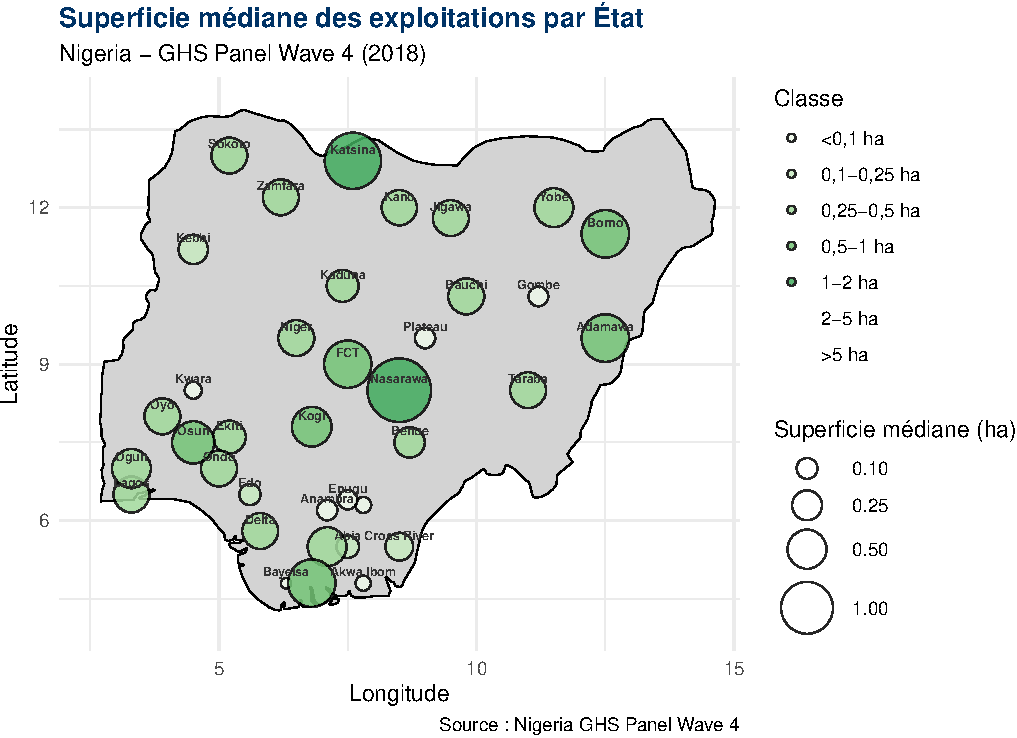
\includegraphics[width=1\linewidth]{rapport_final_files/figure-latex/trend-heatmap-1} \caption{Carte et classement des superficies médianes par État --- Nigeria GHS W4}\label{fig:trend-heatmap-1}
\end{figure}
\begin{figure}[H]
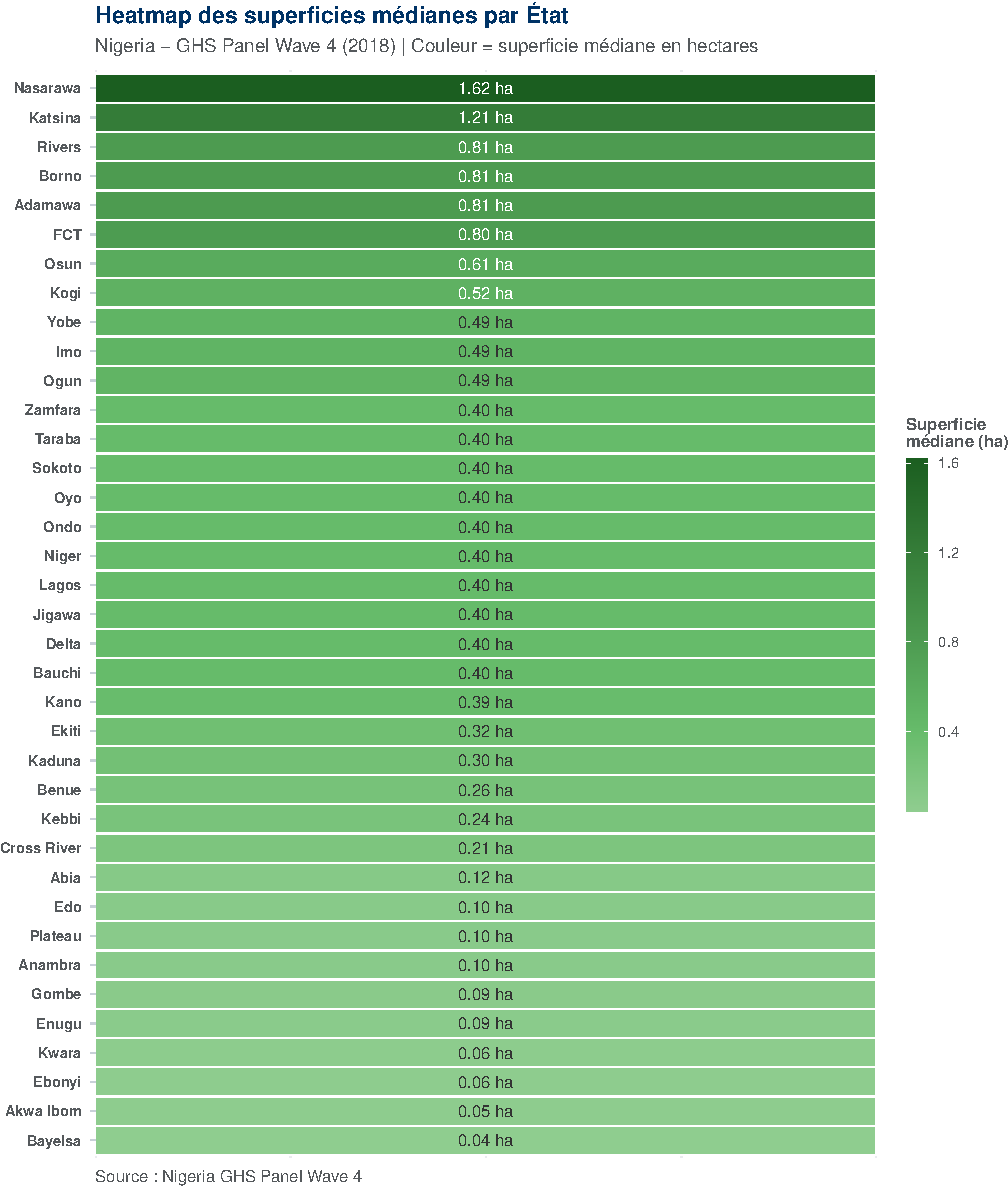
\includegraphics[width=1\linewidth]{rapport_final_files/figure-latex/trend-heatmap-2} \caption{Carte et classement des superficies médianes par État --- Nigeria GHS W4}\label{fig:trend-heatmap-2}
\end{figure}

\section{Conclusion et recommandations}\label{synthese}

Cette étude aboutit à cinq résultats clés. Premièrement, les superficies
agricoles nigérianes présentent une asymétrie positive extrême : la
majorité des ménages cultivent moins d'un hectare, tandis qu'une
minorité d'exploitants concentre l'essentiel des terres. Deuxièmement,
la comparaison entre déclarations orales et mesures GPS révèle une
surestimation systématique par les exploitants (biais médian de -0,0264
ha), avec 38,7 \% des parcelles sous-estimées. Troisièmement, le régime
de tenure dominant est l'héritage (58,2 \%), témoignant de la
persistance des systèmes coutumiers. Quatrièmement, la fragmentation des
exploitations est modérément corrélée à la superficie totale
(\(\rho =0,433\)), avec une progression décroissante au-delà de 8 à 10
parcelles. Cinquièmement, les disparités géographiques Nord-Ouest -
Sud-Est sont très marquées.

\end{document}
